\section{Results and discussion}\label{results}
This section presents the results of the conducted Austrian case study in 2050. Four different storylines are investigated, covering a wide range of possible future developments of the Austrian energy system in the context of European deep decarbonization. Section \ref{res:1} shows the heat generation mix of the supply of the residential and commercial heat demand on the country level. Section \ref{res:2} provides a finer scale and presents the heat generation mix on the sub-region and small-subregion level. Section \ref{res:3} presents the potentials of centralized heat supply on the sub-region level. Section \ref{res:4} shows the centralized heat networks on the small sub-region level. Finally, Section \ref{res:5} compares the obtained centralized heat networks in 2050 with today's networks using heat density as the criterion.

\subsection{Heat supply of the Austrian residential and commercial sector in 2050: four different decarbonization scenarios obtained from the H2020 project openENTRANCE}\label{res:1}
This section presents the heat generation mix covering the Austrian residential and commercial heat demand in 2050 for four different storylines, which were (\textit{or "are currently"}) developed within the H2020 openENTRANCE project. They are named as follows: \textit{Directed Transition}, \textit{Societal Commitment}, \textit{Techno-Friendly}, and \textit{Gradual Development}. Within each of them, specific fundamental development of the energy systems is described while aiming for a sustainable transition of the provision of energy services. The first three storylines consider the achievement of the \SI{1.5}{\degreeCelsius} global warming climate target. The latter storyline (\textit{Gradual Development}) can be interpreted as a more conservative storyline and takes into account the \SI{2.0}{\degreeCelsius} target. Below, the storylines are briefly described before the quantitative results on the country level are presented. For a more detailed description of the storylines, it is referred to \cite{auer2020quantitative} and \cite{auer2020development}. Further informations also are available at the website of the project \footnote{\url{https://openentrance.eu/}} and GitHub.\footnote{\url{https://github.com/openENTRANCE}}.\newline

The underlying concept of the four storylines is a three-dimensional space spanned by the following parameters: technology, policy, and society. Each storyline describes a specific pathway to reach a decarbonized energy system taking into account a pronounced contribution of two dimensions. Regarding the third dimension, a development is assumed that leads to no significant contribution to the decarbonization of the energy system. 

\begin{itemize}
	\item \textit{Directed Transition} looks at a sustainable provision of energy services through strong policy incentives. This bundle of actions becomes necessary because neither the markets nor society adequately pushes sustainable energy technologies.
	\item \textit{Societal Commitment} achieves deep decarbonization of the energy system by a strong societal acceptance of the sustainable energy transition. Thereby, decentralized renewable energy technologies together with policy incentives lead to a sustainable supply of energy service needs. Parallel, no fundamental breakthroughs of new clean technologies are within sight.
	\item \textit{Techno-Friendly} describes a development of the energy system where a significant market-driven breakthrough of renewable energy technologies gives rise to the decarbonization of energy service supply. Alongside, society acceptance supports the penetration of clean energy technologies and the sustainable transition.
	\item \textit{Gradual Development} differs from the other storylines as on the one hand, this storyline only aims for the less ambitious \SI{2.0}{\degreeCelsius} climate target, and on the other hand, a little of each possible sustainable development of the energy system is described here. While all three dimensions contribute to decarbonization, they do not push it sufficiently and result in a more conservative storyline than the others.
\end{itemize}

Table \ref{tab:1} shows the heat generation by technology/source in Austria 2050 for the four different storylines. As mentioned, these values are obtained from the H2020 project openENTRANCE and are the modeling results from the open-source model GENeSYS-MODv2.0 \cite{burandt2018genesys}. According to the underlying assumptions in the storylines, the heat generation of the different sources/technologies vary in some cases significantly (e.g., hydrogen-based heat generation in \textit{Directed Transition} and \textit{Gradual Development} (\SI{7.62}{TWh}) or Heat pump (ground) generation in \textit{Techno-Friendly} and \textit{Societal Commitment} (\SI{14.78}{TWh})). The gray-colored column $\Sigma$) presents the sum of heat generation using centralized heat networks, which varies between \SI{19.49}{} (\textit{Techno-Friendly}) and \SI{35.23}{TWh} (\textit{Gradual Development}).

\newcolumntype{R}[2]{%
	>{\adjustbox{angle=#1,lap=\width-(#2)}\bgroup}%
	l%
	<{\egroup}%
}
\newcommand*\rot{\multicolumn{1}{R{45}{1em}}}
\newcommand*\rots{\multicolumn{1}{R{90}{1em}}}
\definecolor{Gray}{gray}{0.85}

\begin{table}[h] \centering
	\scalebox{0.9}{
	\renewcommand{\arraystretch}{1.35}
	\begin{tabular}{clcccccccc}
		\multicolumn{2}{c}{\thead{Heat generation\\by source in \SI{}{TWh}}} & \rot{Biomass} & \rot{Direct Electric} & \rot{Synthetic gas} & \rot{Heat pump (air)} 
		& \rot{Heat pump (ground)} & \rot{Heat storage} & \rot{Hydrogen} & $\Sigma$\\
		\midrule
		\parbox[t]{2mm}{\multirow{4}{*}{\rotatebox[origin=c]{90}{\small Storyline}}}
		& Directed Transition             & 5.37 & 2.13  & 0.36  & 22.73  & 19.50  & 14.84  & 1.03  & \cellcolor{Gray}25.90\\
		& Societal Commitment               & 5.37 & 1.98 & 1.35 & 15.71 & 21.47 & 10.58 & 2.18 & \cellcolor{Gray}29.02\\
		& Techno-Friendly              & 5.37 & 1.53  & 2.79  & 25.95  & 6.69 & 16.36 & 7.43  & \cellcolor{Gray}19.49\\
		& Gradual Development & 5.37 & 1.81 & 5.35 & 9.68 & 21.21 & 15.57  & 8.65 & \cellcolor{Gray}35.23\\
		\bottomrule
	\end{tabular}}
	\caption{Heat generation by source in TWh supplying the residential and commercial heat demand in Austria 2050 for the different scenarios. Values obtained from the H2020 project openENTRANCE and GENeSYS-MOD.}
	\label{tab:1}
\end{table}

\subsection{Heat technology generation in 2050 on different spatial granularities}\label{res:2}
Figure \ref{fig:res1} shows the heat generation per technology/source on different the country (NUTS0), sub-region (NUTS3) and small sub-region (LAU) level (from left to right). Thus, the level of spatial details increases from the left to the right. In the middle, the residential and commercial heat supply in a representative rural and urban sub-region, respectively, is presented. The rural sub-region (NUTS3 code AT121 (Mostviertel-Eisenwurzen)) shows high shares of heat pumps (air sourced) and small-scale heat storage systems. In addition, synthetic gas and direct electric heating systems supply the heat demand. The urban sub-region (NUTS3 code AT127 (South Viennese environs)) is mainly supplied by ground-sourced heat pumps, biomass, and hydrogen. Air-sourced heat pumps and again heat storage cover the remaining demand. Throughout the figure, shares of heat generation using centralized heat networks are marked by the blue-colored edge. On the very right, an example of the resulting centralized heat network on the small sub-region level for the four different scenarios is presented. In the four subfigures presenting centralized heat networks (each for one storyline), the size of the points indicates the amount of centralized heat supply in a specific small sub-region. The comparably high demand in the \textit{Gradual Development} scenario results in an extensive centralized heat network infrastructure (see lower right subfigure in Figure \ref{fig:res1}). The other three centralized heat networks are characterized by fewer (less supplied small sub-regions) and smaller points (less supplied heat demand by the centralized heat network). Heat generation per technology in Austria 2017 can be found in \ref{appendixA}.

\begin{sidewaysfigure}
	\centering
	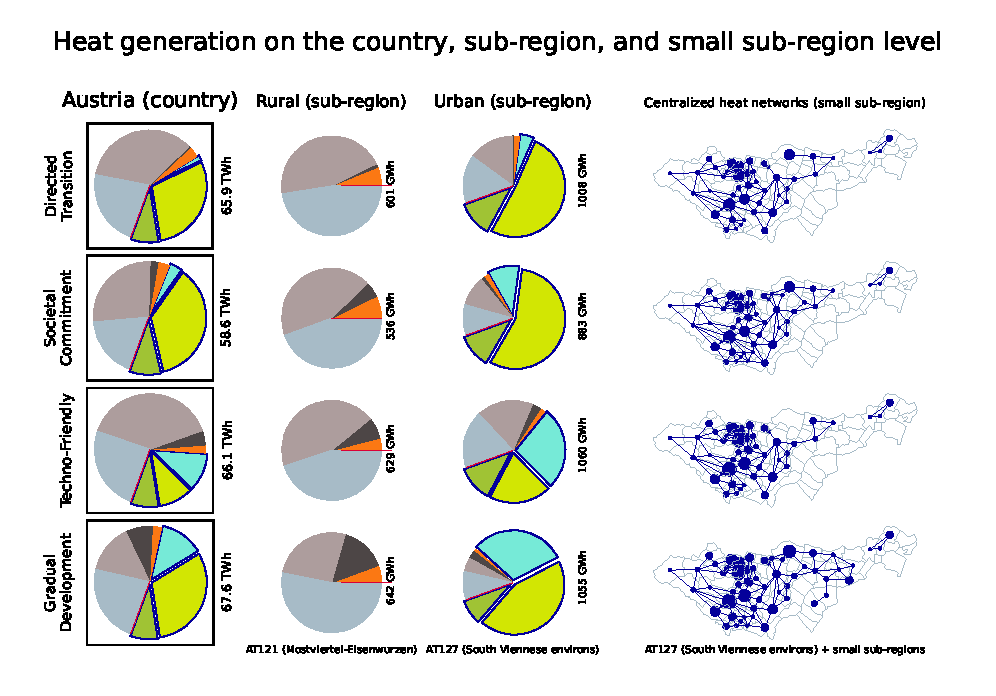
\includegraphics[width=1\linewidth]{figures/4_Results/Spatial_results.eps}
	\caption{Heat technology generation on different spatial granularity levels in the different scenarios supplying the residential and commercial heat demand. left: on the country level. middle: comparison of a rural and urban sub-region. right: centralized heat network topology (size of the points represent the amount of heat demand supplied by the network)}
	\label{fig:res1}
\end{sidewaysfigure}

\subsection{Sub-regions in Austria 2050 with high potentials for centralized heat supply}\label{res:3}
As already indicated in Figure \ref{fig:res1}, the potentials of centralized heat supply in Austria 2050 is limited. In particular, only six different sub-regions (NUTS3 regions) are supplied by heat networks (see Figure \ref{fig:res2}). Although the exact numerical numbers differ, the six sub-regions in each scenario are (partially) supplied by centralized heat networks. Table \ref{tab:3} shows the centralized and on-site heat supply in these six sub-regions. Thereby, the connection rate is assessed by the share of centralized heat supply in the total heat demand. The population density varies in the six sub-regions between \SI{229}{persons \per \kilo\metre^2} (AT323 - Salzburg and sourroundings) and \SI{5124}{persons \per \kilo\metre^2} (AT130 - Vienna).

\begin{table} \centering
	\scalebox{1}{
		\renewcommand{\arraystretch}{1.35}
		\begin{tabular}{cccccc}
			\toprule 
			&& \multicolumn{2}{c}{in TWh} & in \%\\\cmidrule(lr){3-5}
			Sub-region & Storyline&Centralized & On-site & Connection rate\\\hline
			\parbox[t]{2mm}{\multirow{4}{*}{\rotatebox[origin=c]{90}{AT127}}} & Directed Transition & 0.72 & 0.17 & 81\\
			 & Societal Commitment & 0.78 & 0.11 & 88\\
			 & Techno-Friendly & 0.90 & 0.24 & 79\\
			 & Gradual Development & 1.20 & 0.09 & 93\\\hline
 			\parbox[t]{2mm}{\multirow{4}{*}{\rotatebox[origin=c]{90}{AT130}}} & Directed Transition & 3.98 & 0.95 & 81\\
			 & Societal Commitment & 4.28 & 0.61 & 88\\
			 & Techno-Friendly & 4.98 & 1.33 & 79\\
			 & Gradual Development & 6.59 & 0.47 & 93\\\hline
			  \parbox[t]{2mm}{\multirow{4}{*}{\rotatebox[origin=c]{90}{AT221}}} & Directed Transition & 0.92 & 0.22 & 81\\
			 & Societal Commitment & 1.53 & 0.14 & 92\\
			 & Techno-Friendly & 1.16 & 0.31 & 79\\
			 & Gradual Development & 1.53 & 0.11 & 93\\\hline
			 \parbox[t]{2mm}{\multirow{4}{*}{\rotatebox[origin=c]{90}{AT312}}} & Directed Transition & 1.24 & 0.30 & 81\\
			 & Societal Commitment & 1.34 & 0.19 & 88\\
			 & Techno-Friendly & 1.56 & 0.42 & 79\\
			 & Gradual Development & 2.06 & 0.15 & 93\\\hline
			  			\parbox[t]{2mm}{\multirow{4}{*}{\rotatebox[origin=c]{90}{AT323}}} & Directed Transition & 0.75 & 0.18 & 81\\
			 & Societal Commitment & 1.24 & 0.11 & 92\\
			 & Techno-Friendly & 0.93 & 0.25 & 79\\
			 & Gradual Development & 1.24 & 0.09 & 93\\\hline
			  			\parbox[t]{2mm}{\multirow{4}{*}{\rotatebox[origin=c]{90}{AT342}}} & Directed Transition & 0.66 & 0.16 & 81\\
			 & Societal Commitment & 0.71 & 0.10 & 88\\
			 & Techno-Friendly & 0.82 & 0.22 & 79\\
			 & Gradual Development & 1.09 & 0.08 & 93\\\hline
			 & & \multicolumn{2}{c}{Average connection rate}& \SI{85.25}{\%}\\
			\bottomrule
	\end{tabular}}
	\caption{Centralized heat supply and on-site heat generation in the six Austrian sub-regions, with potentials of centralized heat networks in 2050}
	\label{tab:3}
\end{table}

\begin{sidewaysfigure}
	\centering
	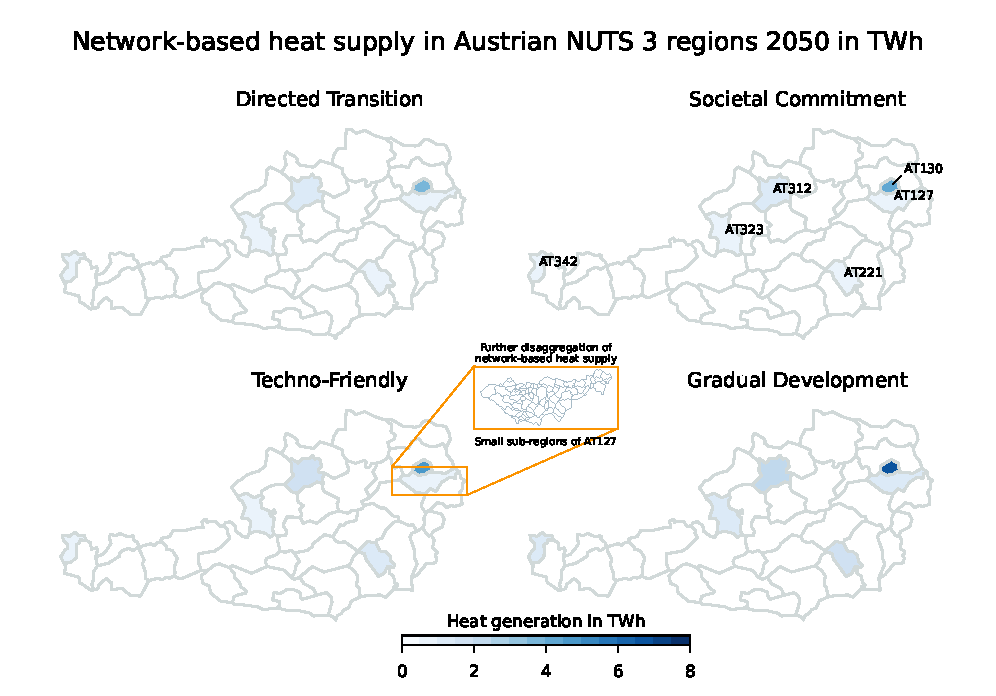
\includegraphics[width=1\linewidth]{figures/4_Results/Heatmap.eps}
	\caption{Centralized heat supply in Austria 2050}
	\label{fig:res2}
\end{sidewaysfigure}

\newpage
\subsection{Centralized heat network topology on the small sub-region level}\label{res:4}
This section presents the centralized heat network topology of the sub-region AT127 (including all small sub-regions). Note that this is the highlighted sub-region in Figure \ref{fig:res2} marked by the orange box. Figure \ref{fig:res3} shows the results of the iterative downscaling algorithm. The number of small sub-regions supplied by the centralized heat network is plotted on the horizontal axis. Note that this number decreases from left to right. The blue-marked area highlights the initial state of the centralized heat network ($G^{0}$). The boxplot illustrates the distribution of the indicator values benchmarking the network graph. It becomes visible that by removing small sub-regions, namely iteratively those with the smallest indicator value, the mean indicator value of the entire remaining heat network increases. In addition, the maximum value of the indicator also increases from under 1.64 to over 7.16. In the present example, the number of small sub-regions supplied by the centralized heat network decreases from \SI{75}{} to \SI{47}{} (\SI{-37.3}{\%}). The green-marked area highlights the improved centralized heat network topology ($G^{*}$). The iterative reduction of supplied small sub-regions does not necessarily result in a contiguous graph. For example, three small sub-regions form a subgraph that is separate from the other network (see upper right in the green box in Figure \ref{fig:res3}). The results discussed above suggest that reducing the number of small sub-regions supplied by the centralized heat network increases the indicator value and thus the efficiency of the heat network topology. Simultaneously, this also increases the heat density of the supply area. In the following subsection, the obtained heat density values of the heat networks are compared with existing values and today's minimum required values for centralized heat networks.

\begin{sidewaysfigure}
	\centering
	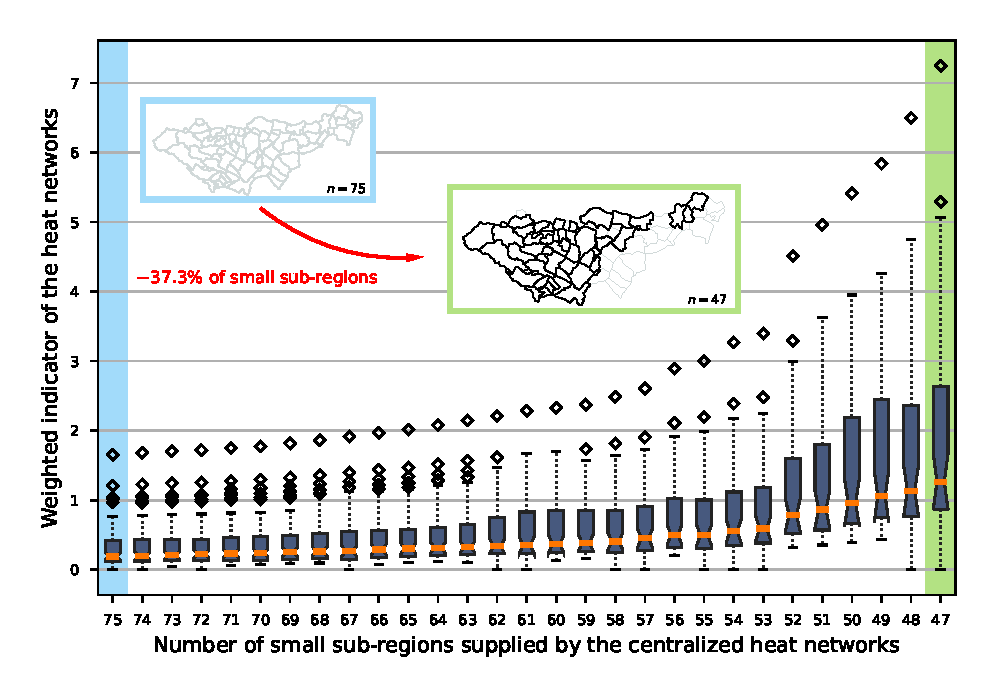
\includegraphics[width=1\linewidth]{figures/4_Results/boxplot.eps}
	\caption{Benchmark indicator value of the centralized heat network at the sub-region AT127 (South Viennese environs) for different numbers of areas supplied.}
	\label{fig:res3}
\end{sidewaysfigure}

\subsection{Comparing centralized heat networks in 2050 with of existing and future projections of low temperature heat networks using heat and population density}\label{res:5}
This section synthesizes the results of the centralized heat network topologies accounting for heat densities. Again, the quantitative results of the sub-region AT221 (Graz, district of Graz environs) are used to illustrate the comparison between the future and today's centralized heat networks. Figure \ref{fig:res4} presents the heat density of the centralized heat network in the sub-region for the three different downscaling techniques. The iterative downscaling algorithm generates the highest heat densities. This downscaling technique increases the heat density of the centralized network by \SI{2.15}{\frac{GWh}{km^2}} compared to population-based downscaling and by \SI{1.08}{\frac{GWh}{km^2}} compared to the sequential downscaling algorithm. However, the gap in heat density compared to today's centralized heat networks becomes apparent. As reference, a heat density of \SI{10}{\frac{GWh}{km^2}} with a connection rate of \SI{90}{\%} is assumed\footnote{\url{http://www.austrian-heatmap.gv.at/ergebnisse/}}. The gap of heat density varies between the different scenarios. The smallest is achieved in the \textit{Directed Transition} scenario and amounts to \SI{7.42}{\frac{GWh}{km^2}}. The highest value is \SI{8.41}{\frac{GWh}{km^2}} in the \textit{Societal Commitment} scenario. Figure \ref{fig:res5} below shows the heat density of centralized heat networks in the different sub-regions. 
\begin{figure}[h]
	\centering
	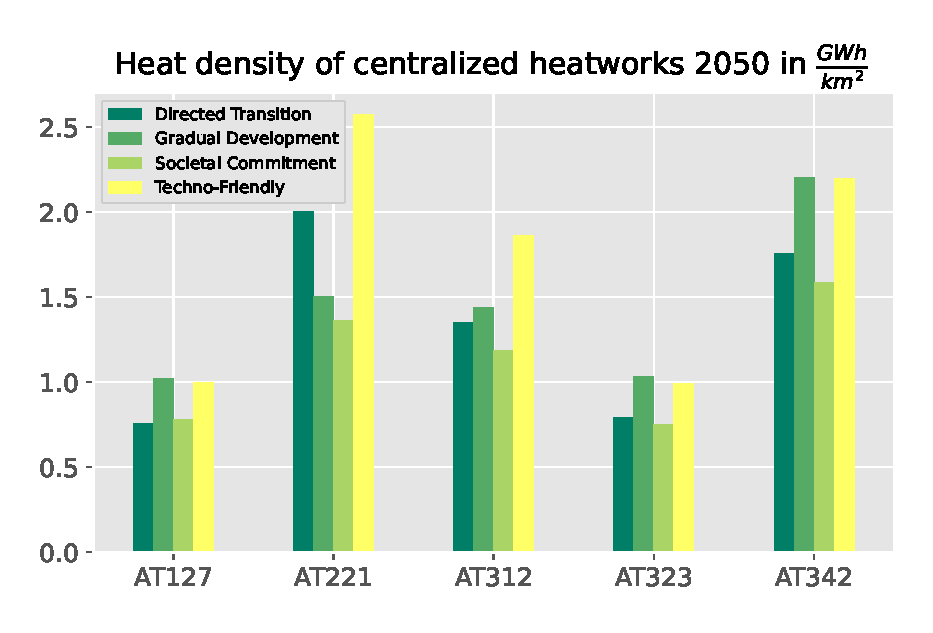
\includegraphics[width=0.95\linewidth]{figures/4_Results/plot.eps}
	\caption{Heat densities of centralized heat networks at the sub-region level for the different scenarios}
	\label{fig:res5}
\end{figure}

The \textit{Techno-Friendly} scenario shows the highest values of obtainable heat densities in the sub-regions. For reasons of clarity, the values for AT130 (Vienna) are not shown in the figure. These amount to \SI{9.6}{\frac{GWh}{km^2}} in the \textit{Directed Transition}, \SI{10.3}{\frac{GWh}{km^2}} in the \textit{Societal Commitment}, \SI{12.0}{\frac{GWh}{km^2}} in the \textit{Techno-Friendly}, and \SI{15.9}{\frac{GWh}{km^2}} in the \textit{Gradual Development} scenario.

\begin{sidewaysfigure}
	\centering
	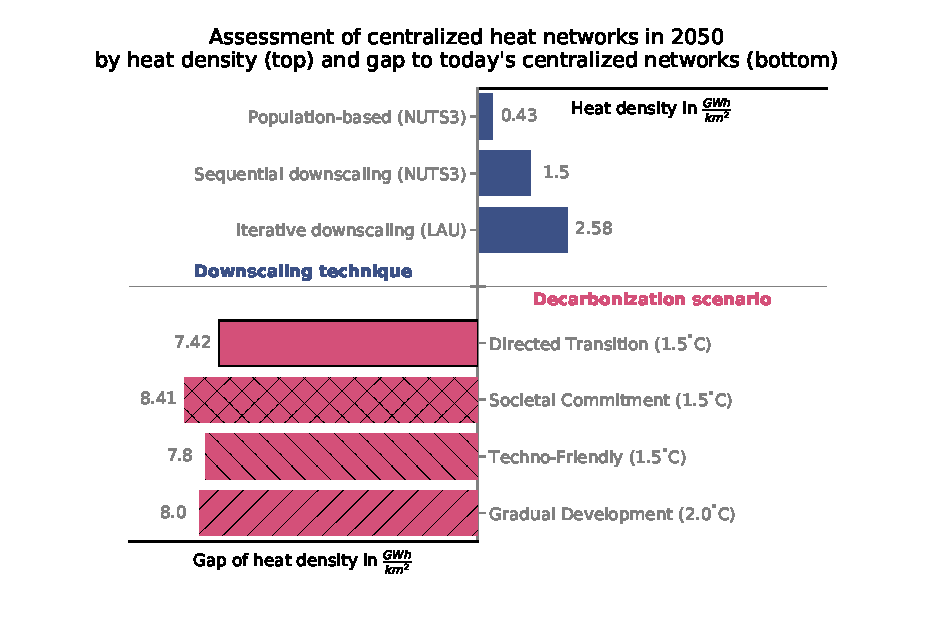
\includegraphics[width=1\linewidth]{figures/4_Results/HD.eps}
	\caption{Heat density obtained by the different downscaling techniques (top) and heat density gap between centralized heat networks in 2050 and today for the four different scenarios. Numerical values shown for the sub-region AT221.}
	\label{fig:res4}
\end{sidewaysfigure}